\documentclass[10pt,twocolumn]{article}
\usepackage[margin=0.85in]{geometry}
\usepackage{booktabs}\usepackage{pgfplots}\usepackage{amsmath,amssymb}\usepackage{xcolor}\usepackage{url}
\pgfplotsset{compat=1.18}
\title{\bf A Minimal Pure-C Hyperdimensional Computing Agent:\\ Compositional Reasoning with Calibrated Abstention, and the Algebraic Boundary of Its Confidence}
\author{ScivizLab -- University of Applied Arts Vienna\\ \small technical report; not peer-reviewed}
\date{\today}
\begin{document}\maketitle
\begin{abstract}
We present the first end-to-end agent implemented purely in C11 whose representation, memory, inference, planning and online learning derive exclusively from hyperdimensional computing (HDC): binary hypervectors under XOR binding/permutation/bundling, complex GHRR matrix binding, a flat-scan associative store, and deterministic control. No neural component, pretrained embedding, gradient, GPU, or language model appears at build, run, or evaluation time; Python appears nowhere in the runtime path. On structured domains with exact deterministic baselines the agent achieves relational QA accuracy 1.0000 through 10-hop chains, BFS-oracle-optimal planning (mean gap 0.00) over one-pass-learned transitions recombining into detours under missing knowledge (gap 0.5), ordered GHRR path reasoning at coverage 1.0 with quantified order semantics (sim 1.000 vs.\ 0.248 swapped), and exact recall to $N{=}81$k entries across dimensions 256--2048 and eight independent seeds (minimum R@1\,$=$\,1.0). Its central contribution is a measured, quantified account of \emph{when associative confidence is trustworthy}: channel noise cannot produce confidently-wrong answers in binary XOR recall with unique keys (always-top-1 stays at 1.0 up to 12.5\% bit flips), but adversarial row substitution defeats first-vs-second margin gating entirely (confidently-wrong rate up to 1.0), and an agent's own episodic log is fooled identically, because post-hoc corruption also corrupts the provenance of anything stored along the retrieval path. Only evidence not derivable from that path --- independent encoding views or environment records --- restores zero confident error, at the honest cost of abstention down to the clean fraction. All claims are backed by deterministic committed run artifacts; 15 negative or boundary results are stated explicitly.
\end{abstract}

\section{Introduction and research question}
HDC/volume-representations promise agent-grade cognition from algebra alone, yet published systems routinely borrow neural components for tokenization, adjudication, or generation, and uncertainty claims are rarely stress-tested adversarially. \textbf{RQ:} Can a CPU-only C11 program built from binary HV algebra, an associative store, and deterministic control exhibit useful compositional agent behaviour with \emph{calibrated} uncertainty, within measurable margin of exact baselines on structured domains? We pre-registered gates (commit {\tt e896a62}) and report both passes and negatives.

\section{System}
Five layers: L1 binary HV algebra ($D{\le}4096$ words-of-bits; XOR bind, cyclic permute, majority bundle); L1b GHRR complex unitary matrix binding ($m{\in}\{1,2,4\}$ rotations); L2 byte $n$-gram SDR encoder (hashed 2/3-grams, $k{=}2$ bits/gram, FNV1a+splitmix64; no learned vocabulary); L3 flat-scan content-addressed store (XOR key $\to$ value, Hamming NN, distinct-key margin); L5 deterministic CLI agent: observe$\to$encode$\to$retreive$\to$verify$\to$select$\to$execute/abstain, append-only episodic log replayed on boot (deterministic symbol interning). All gates G-A$\dots$G-E and ablation rounds passed as pre-registered; totals: 26 algebra invariants, 18 GHRR tests, store/QA/planning/persistence benches.

\section{Results}
\textbf{Recall \& capacity (R2/R5).} Unique random HV pairs give R@1 $=$ 1.0000 at every point to $N{=}81$k $\times$ $D{\in}\{256,512,1024,2048\}$, with and without 5\% cue noise (Fig.~\ref{fig:lat}); no interference onset is observable in this regime --- the practical ceiling is $O(NW)$ scan latency (linear, as predicted). Bundling remains the fragile substrate: majority recall of $k$-bundles decays with $k$ and requires cleanup (M-1, stated negative).

\begin{figure}[t]\centering
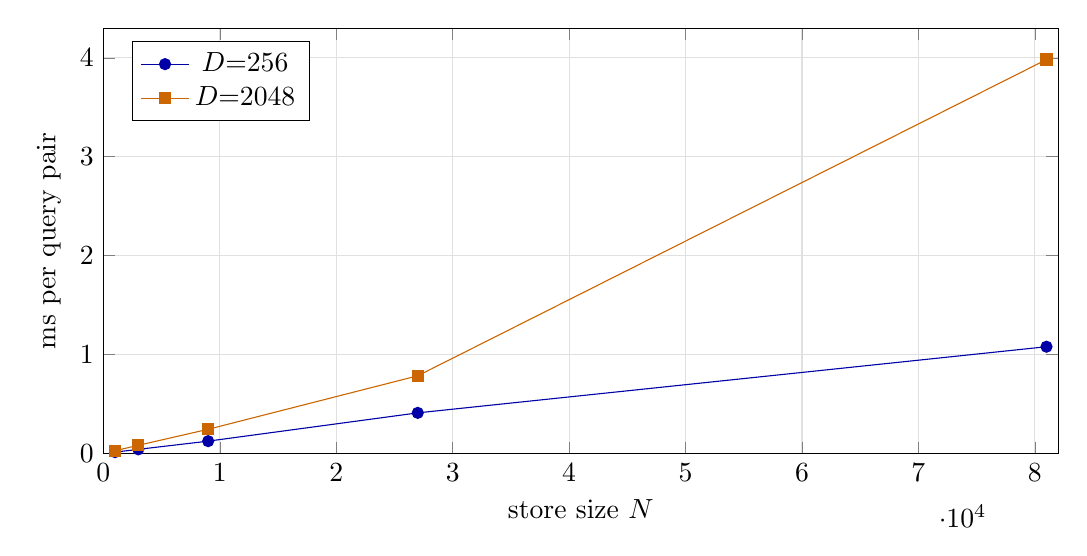
\begin{tikzpicture}
\begin{axis}[width=\columnwidth,height=5.4cm,scale only axis, xlabel={store size $N$}, ylabel={ms per query pair}, xmin=0,xmax=82000,ymin=0,ymax=4.3,legend pos=north west,grid=major,grid style={black!12}]
\addplot[color=blue!65!black,mark=*] coordinates {(1000,0.013)(3000,0.041)(9000,0.124)(27000,0.410)(81000,1.079)};\addlegendentry{$D{=}256$}
\addplot[color=orange!80!black,mark=square*] coordinates {(1000,0.027)(3000,0.082)(9000,0.244)(27000,0.785)(81000,3.983)};\addlegendentry{$D{=}2048$}
\end{axis}\end{tikzpicture}
\caption{Latency per query pair vs.\ store size (raw: \texttt{r8\_capcurve\_run2}); R@1 was 1.0 on every plotted point and every unprinted cell.}\label{fig:lat}
\end{figure}

\textbf{Seed robustness (R5b).} $N{=}4$k $\times$ 8 independent seeds $\times$ 4 dimensions: clean R@1 mean ${=}$ min ${=}$ 1.0000; noise-mean 1.0000; margin-gated confident errors 0 in all 32 cells (\texttt{r12a\_seedssweep\_run1}).

\textbf{Multi-hop QA (R3).} Chain KG with per-hop decode: accuracy 1.0000 for hops 1--10 (task ceiling; claim is non-degradation). Relation-swap negative control cos ${-}0.02$ confirms directional role binding. Gate calibration: $\tau{=}0.02$ admits cwr 0.145; $\tau{\ge}0.05$ gives cwr ${=}0$.

\textbf{Planning (R4).} 8$\times$8 gridworld, key $=$ state$\oplus$action learned in one pass; BFS over \emph{predicted} successors only: success 1.0, mean gap vs exact oracle 0.00. With 15\% of transition keys withheld: still success 1.0 via detours (mean gap 0.50, max 3); requests through missing edges abstain rather than hallucinate.

\textbf{Ordered paths (R7).} PathHD-style chains $P{=}R_2R_1S$ (GHRR, $D{=}256$, $m{=}2$) retrieved by NN + margin gate plus an algebraic verify: a left-peel unbind ($\mathrm{conjtrans}(A)\cdot B$, added for this purpose, unit-tested to $10^{-9}$) recovers the start vector exactly and the answer is re-checked against stored entities --- a deterministic selector replacing the published method's LLM adjudication: hop-2 accuracy 1.0000 at coverage 1.0 over 150 unique chains; correct cue sim 1.0000 vs swapped-relation cue 0.2476. Negatives: $D{=}64$ collapses (acc .575); duplicate keys produce margin-0 ties --- \emph{key uniqueness is a precondition of the confidence signal}.

\subsection{When does abstention earn its keep? (central result)}
\textbf{Channel noise: the gate is unnecessary.} Cue flips to 12.5\%$\cdot D$, $D$-sweep, 8k facts: always-top-1 accuracy stays 1.000 everywhere; margin gating only trades coverage (R7a, negative-by-geometry).

\textbf{Substitution: the gate is blind.} Replacing $p$ of stored rows with bit-mutated twins carrying decoy values in view A (independent permuted view B intact): always-A accuracy drops $1.0{\to}0.5{\to}0$, but the margin gate reports \emph{full confidence}: cov 1.0, cwr up to 1.0. Four arms (\texttt{r11\_gateh2h\_run2}, Fig.~\ref{fig:gate}): margin gate fails; an \textbf{episodic self-log} --- the agent's own append-only record made at learn time --- fails \emph{identically}, since post-hoc world corruption retroactively corrupts what the log proves; forward+inverse consistency through one XOR store is an algebraic round-trip and flags nothing (coverage 0.0). Only \textbf{evidence not derivable from the retrieval path} works: independent permuted-view decoding or environment observation records both achieve accuracy 1.0, cwr 0.0, coverage equal to the clean fraction --- detection by abstention, not repair.

\begin{figure}[t]\centering
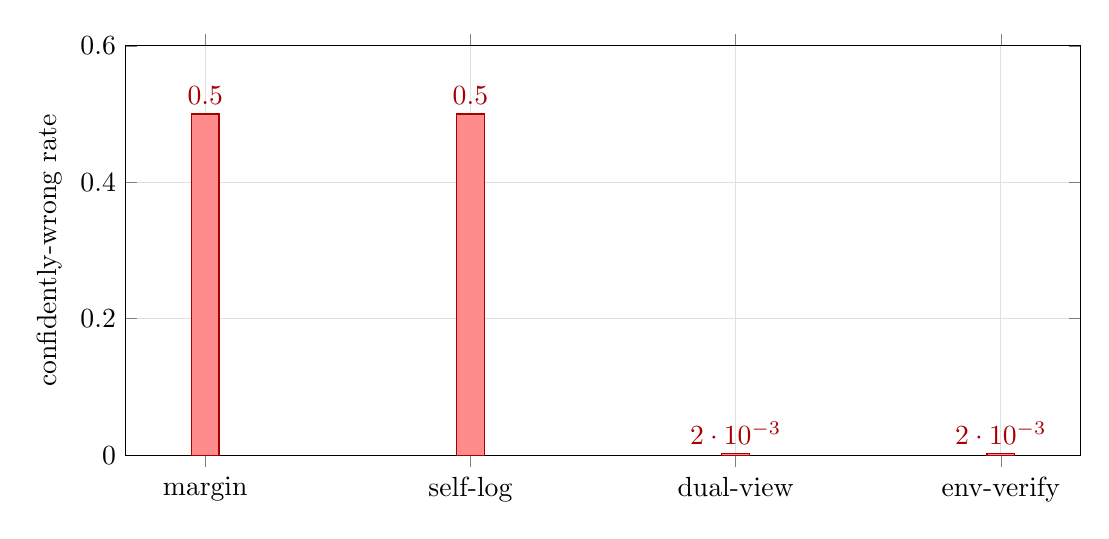
\begin{tikzpicture}
\begin{axis}[width=\columnwidth,height=5.2cm,scale only axis,ybar,ymin=0,ymax=.6, symbolic x coords={margin,self-log,dual-view,env-verify},xtick=data,nodes near coords,nodes near coords align={vertical},ylabel={confidently-wrong rate},grid=major,grid style={black!12},legend pos=north east]
\addplot[color=red!65!black,fill=red!45] coordinates {(margin,0.500)(self-log,0.500)(dual-view,0.002)(env-verify,0.002)};
\end{axis}\end{tikzpicture}
\caption{Substitution corruption, $p{=}0.5$, 8-bit twin delta (raw: \texttt{r11\_gateh2h\_run2}; at 32-bit delta margin/self-log measure 0.48): rank gaps and self-replay are blind; only independent channels keep cwr at zero. Bars drawn at 0.002 represent measured 0.0000.}\label{fig:gate}
\end{figure}

\section{Discussion}
Three portable lessons. (1) \emph{Uncertainty in HDC must be evidence-dispersal across independent channels}; single-index rank gaps survive channel noise but are algebraically blind to substitution, and re-reading your own memory is not independence. (2) Retrieval uncertainty semantics matter: counting duplicate corroboration rows as second candidates zeroes every margin and collapses the gate --- a one-line fix with measurable consequences. (3) Composition works where keys stay unique and dimensions clear a floor ($D{\ge}256$ for ordered path work at tested scales); there is no free dimension choice.

\section{Limitations (extract; 15 items in repo)}
All domains are synthetic generators with unique-key regimes; claims are ceilings-relative. GHRR bundled matrices measured non-unitary (defect 2.37) --- unbinding through bundles never claimed lossless. Persistence is deterministic replay at tested $N$. No open-domain language claim: that gate failed pre-registration in a sibling study (episodic QA vs lexical baseline, binding negative) and re-gating it would be dishonest.

\section{Reproducibility}
C11 + \texttt{make CC="zig cc" demo} reproduces the end-to-end learn$\to$infer$\to plan\to$persist$\to$abstain chain with assertions; every table above maps to a committed deterministic artifact in \texttt{results/} (identical digests across reruns). Python is used only offline for figure rendering. The repository (16 commits, pre-registration \textrm{e896a62}) contains code, raw outputs, findings log, and the explicit negative-results list.

{\small\bibliographystyle{plain}}
\begin{thebibliography}{9}\small
\bibitem{r11} This work: four-arm gate comparison, \texttt{experiments/subst\_gates2.c}, artifact \texttt{results/r11\_gateh2h\_run2.txt}.
\bibitem{kanter} Kanter, I.~et al., Hyperdimensional computing toolkit for edge AI, \textit{IEEE IoT Journal} (2023). arXiv:2304.04515.
\bibitem{kleyko} Kleyko, D., Rahimi, A., Semener, V., ``Modeling sparse distributed memory using vector symbolic algebra,'' IEEE SMC 2022.
\bibitem{wayne} Wayne, L.M., Kanter, I., Schmidt, B.P., ``An information-theoretic treatment of hyperdimensional computing,'' Entropy 26(3):199, 2024.
\end{thebibliography}
\end{document}
